\documentclass[a4paper, 11pt]{article}
\usepackage{comment} % enables the use of multi-line comments (\ifx \fi) 
\usepackage{fullpage} % changes the margin
\usepackage{color,listings,graphicx,float,booktabs,multirow, amsmath}
\usepackage[colorlinks=true, urlcolor=blue]{hyperref}

\definecolor{codegreen}{rgb}{0,0.6,0}
\definecolor{codegray}{rgb}{0.5,0.5,0.5}
\definecolor{codepurple}{rgb}{0.58,0,0.82}
\definecolor{backcolour}{rgb}{0.95,0.95,0.92}
 
\lstdefinestyle{mystyle}{
    backgroundcolor=\color{backcolour},   
    commentstyle=\color{codegreen},
    keywordstyle=\color{magenta},
    numberstyle=\tiny\color{codegray},
    stringstyle=\color{codepurple},
    basicstyle=\footnotesize,
    breakatwhitespace=false,         
    breaklines=true,                 
    captionpos=b,                    
    keepspaces=true,                 
    numbers=left,                    
    numbersep=5pt,                  
    showspaces=false,                
    showstringspaces=false,
    showtabs=false,                  
    tabsize=2
}
 
\lstset{style=mystyle}

\begin{document}
\graphicspath{{./figures/}}
\noindent
\large\textbf{Kyle Salitrik} \\
\normalsize CMPSC 450\\
\large{Homework 3 Report} \hfill 

\section*{Algorithms Implemented}
Three different approaches were used to find the sum of the arrays. The first approach is the binary tree PRAM summation. For this approach, the array is divided amongst the number of threads, where each thread computes a set number of two element sums and then places them into an array of size N/2. The function then recurses, passing down this array of N/2 to be summed. Although we know the theoretical parallel time complexity to be $O(log_2 N)$, looking at the serial complexity, the following can be observed:

\begin{align*}
	O(\text{binary\_sum}) = & O(N + \frac{N}{2} + \frac{N}{4} + \dots + \frac{N}{2^i} + \dots + 2) = O(2N-1) = O(N)
\end{align*}

The second approach was to divide the array across the number of processors and sum all elements assigned to that processor, place that partial sum into a scratch array with the size equal to the number of threads, and then sum all of the scratch array elements afterwards. This divide-and-conquer function was named parallel\_sum. When the number of threads is equal to 1, the order

\begin{align*}
		O(\text{parallel\_sum}) &= O(N); p=1 \\
		O(\text{parallel\_sum}) &= O(N/p)
\end{align*}

The third approach is, in theory, identical to the parallel sum approach. By implementing the parallel for reduction method of OpenMP, the array should be split into equal segments per thread, each section added into a temporary sum, and then the actual sum computed by summing all of these partial sums. The time complexity should be the same as that of the previous approach. In practice, however, we will observe that the extra overhead in manually managing the divide-and-conquer method causes the time to be slightly higher than that of the parallel reduction method.

All three approaches were run using 1, 2, 4, 8, 16, 20, and 24 threads. One preliminary result that was interesting is that, even for the divide-and-conquer methods, as the number of threads diverged from powers of two performance was reduced. Using 16 threads had the best performance for all algorithms.

\section*{Algorithm Performance Comparison}
For all of the graphs in this section, time is on the Y axis, the number of array elements is on the X axis and the number of threads is indicated by the legend. This first graph plots the performance of the binary tree summation. For all numbers of threads, the amount of time spiked at $N = ~8,200,000$. As stated before, each power of two increases the performance (which is to be expected), however using 20 threads has a lower performance than even 8 threads and using 24 threads is only slightly better than 8 threads.

\begin{figure}[H]
	\centering
	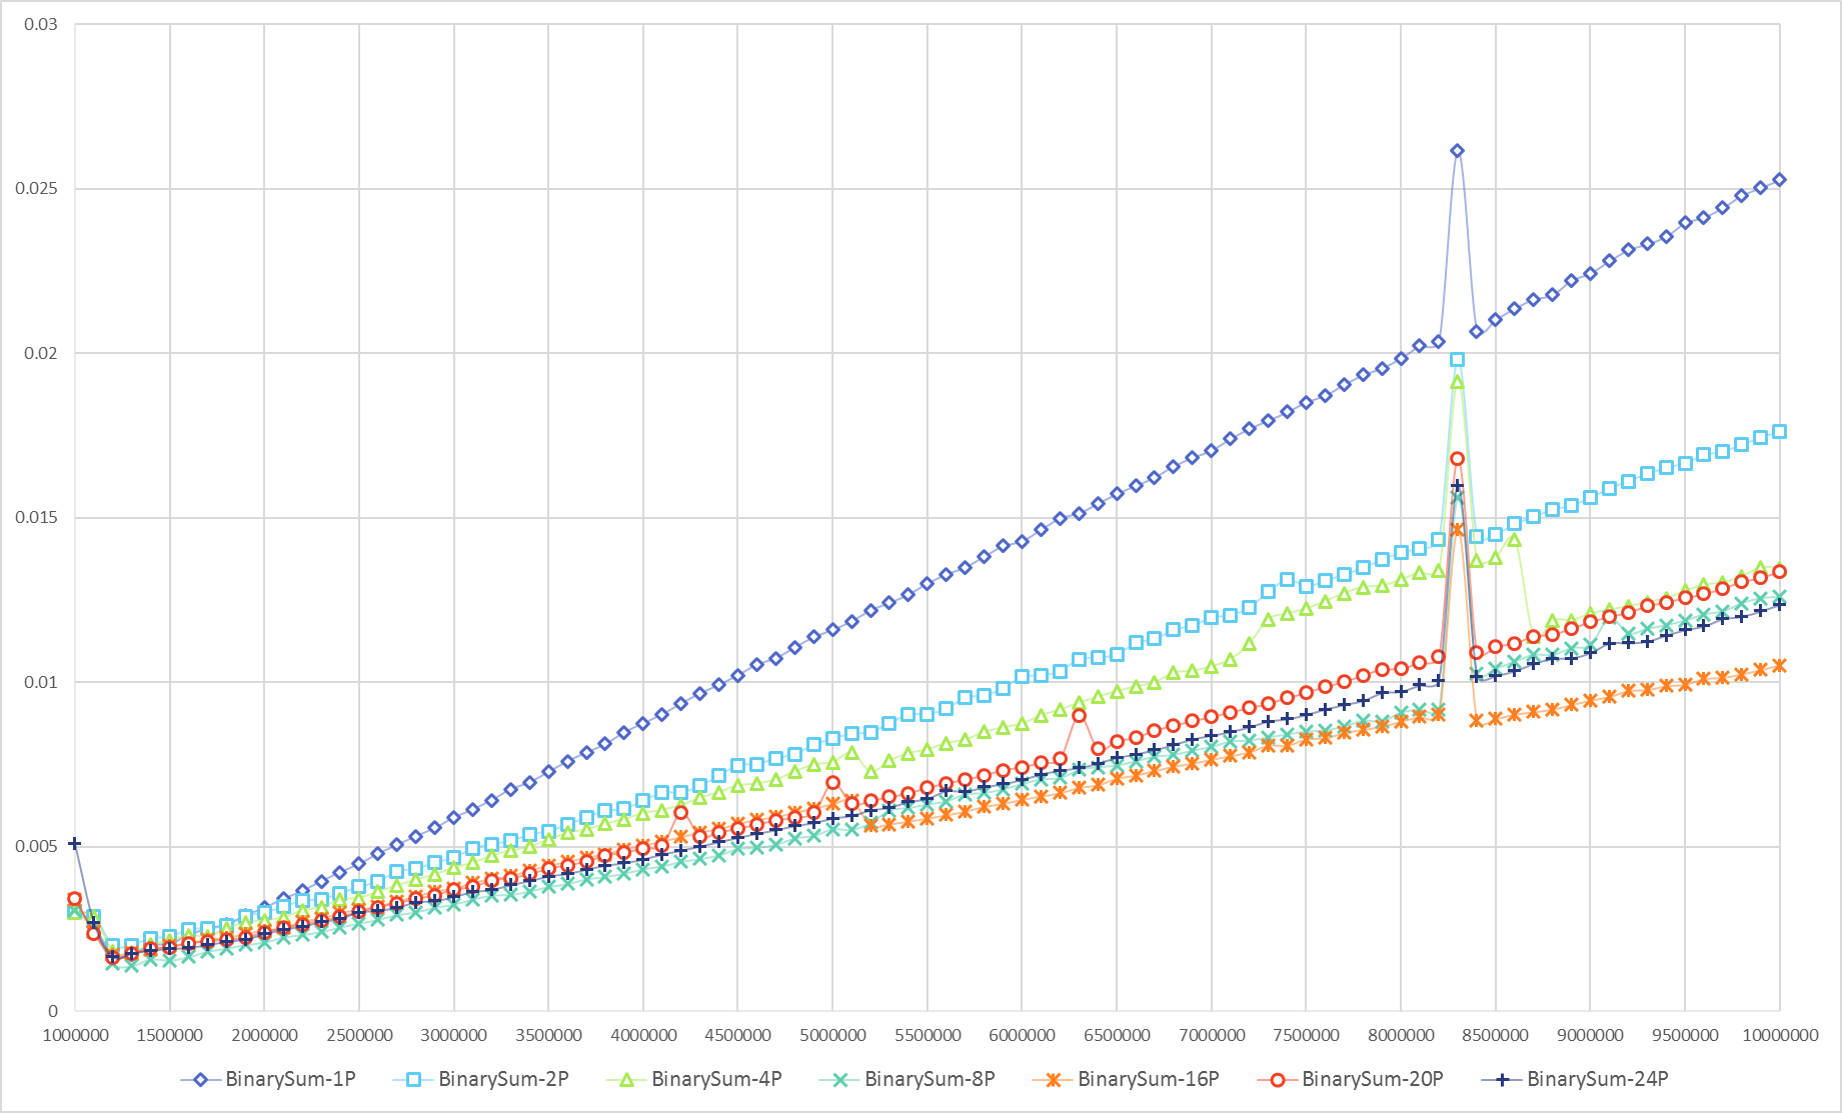
\includegraphics[width=\textwidth]{binary_sum.png}
	\caption{Binary Tree Sum Performance}
\end{figure}

Second up is the parallel sum method. Even in the worst case (1 thread) it is still more than twice as fast as the binary sum method. This follows our realistic expectations of the asymptotic complexity. The time complexity of the serial binary sum is $O(2N-1)$ while the parallel sum method only requires $O(N)$ time. As the number of threads increases, this difference becomes more and more drastic. The same performance spike around 8.2 million is present here as well. It is also worth noting that there is odd behavior when using 4 threads.
\begin{figure}[H]
	\centering
	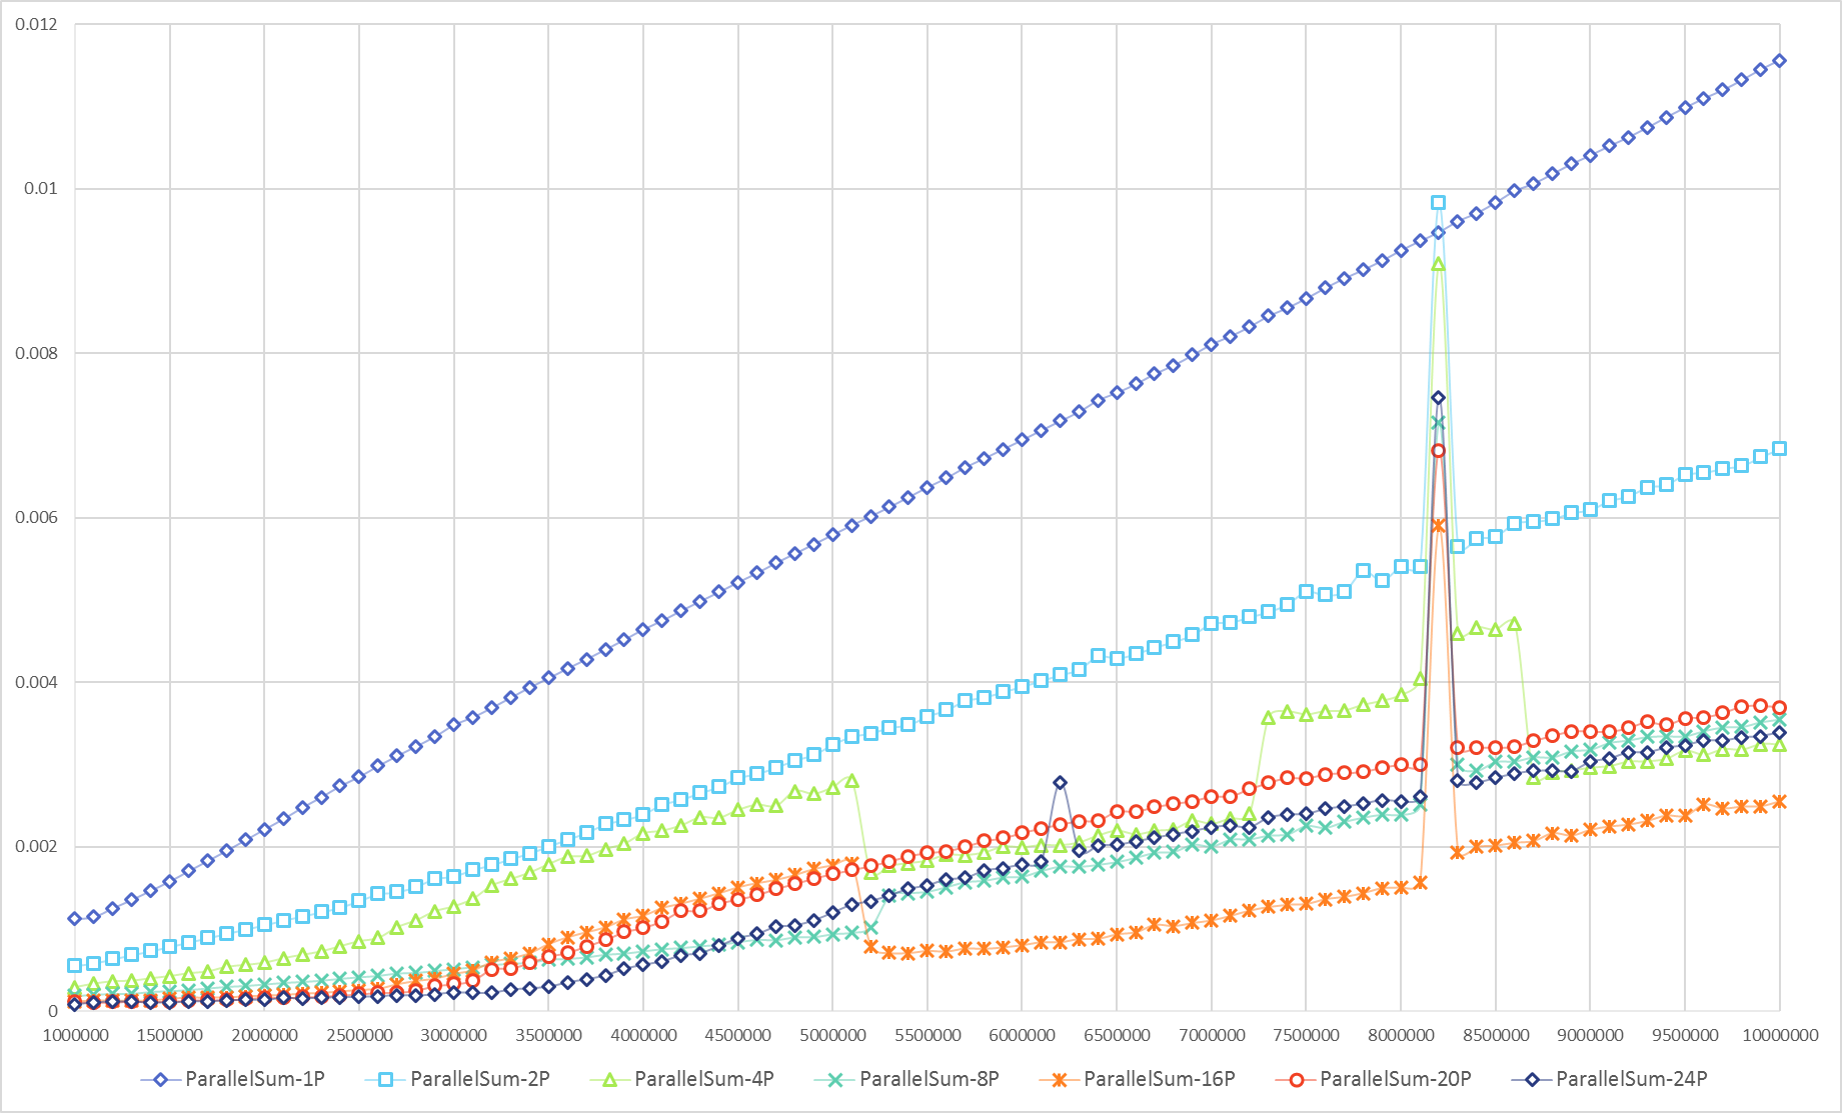
\includegraphics[width=\textwidth]{parallel_sum.png}
	\caption{divide-and-conquer Sum Performance}
\end{figure}

When observing the fast sum method, we see very similar values of time for threads and, as with the previous method, there is odd stepping in performance when using 4 threads. It is worth noting, however, that while in the previous two methods using 20 threads was worse than 8 threads, when using the reduction method, the performance is almost equivalent. The major feature that stands out is that using this method does not cause the peak in performance around 8.2 million elements.
\begin{figure}[H]
	\centering
	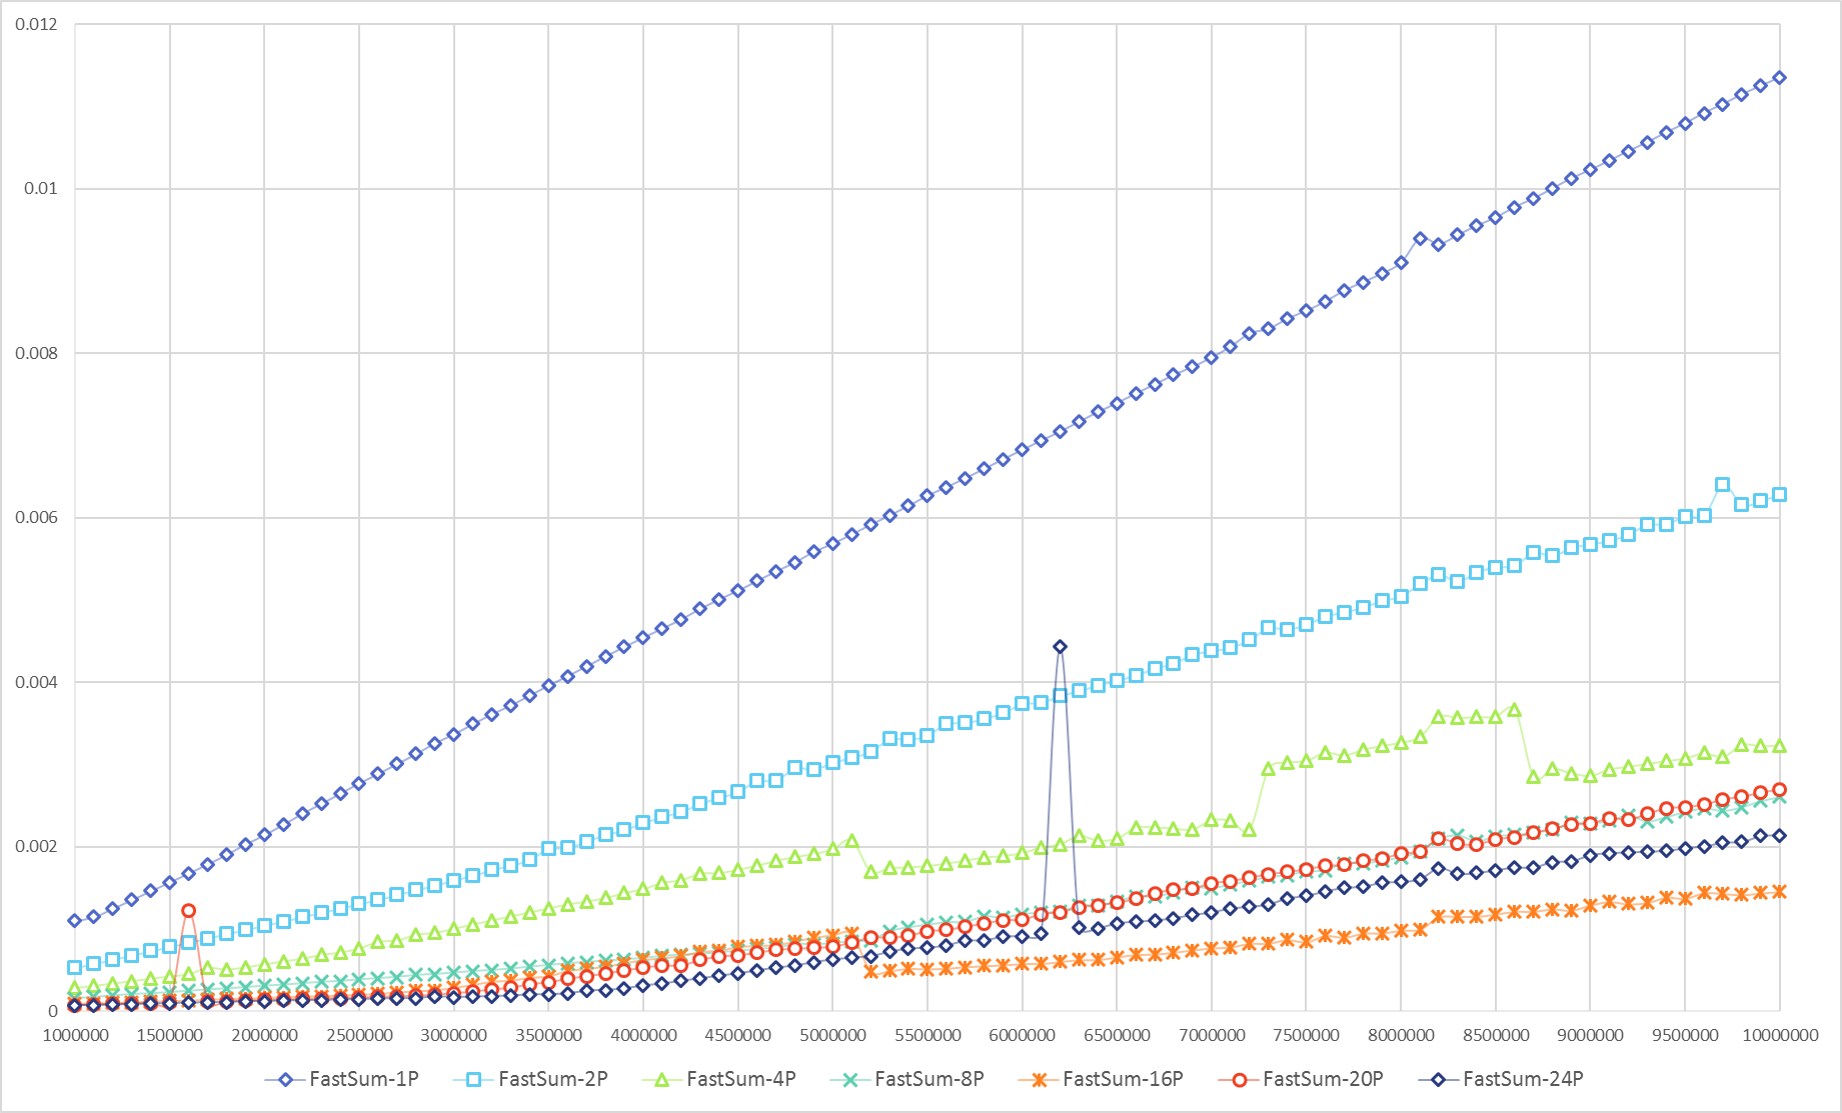
\includegraphics[width=\textwidth]{fast_sum.png}
	\caption{Reduction Sum Performance}
\end{figure}

As a side-by-side comparison of the two methods, the fast sum and parallel sum performances are plotted below. The fast sum values are marked by the dashed line. As expected, by manually managing the shared variables and scratch space used by the parallel method, the performance is slightly worse on all accounts.
\begin{figure}[H]
	\centering
	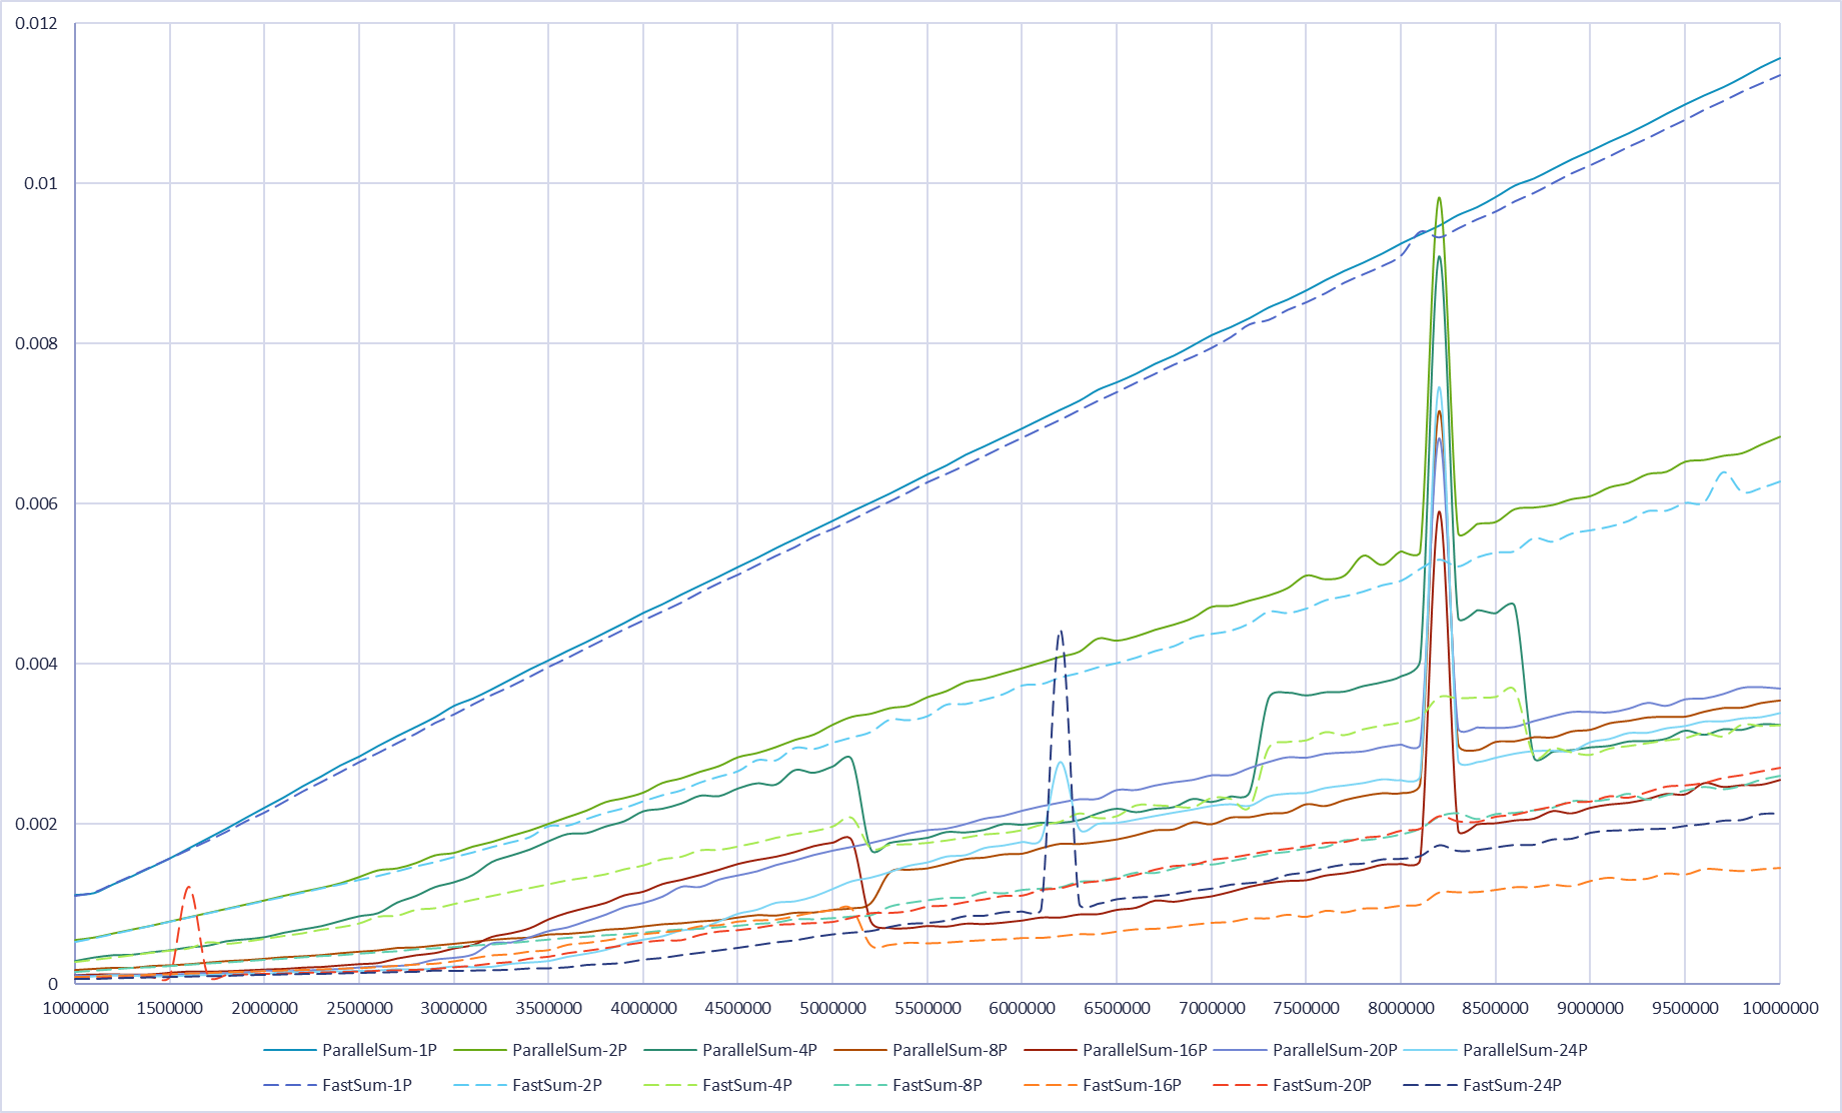
\includegraphics[width=\textwidth]{parallel_vs_fast.png}
	\caption{Parallel vs Fast Sum Performance}
\end{figure}

This graph provides a simple comparison between the serial performance of all three methods. Again, as assumed, the binary sum takes nearly twice the time that the parallel and fast methods do at large N. The management of the scratch space used also takes a toll on $N < 1,300,000$, as can be observed by the significantly higher runtime for these smaller N values in the binary tree sum.
\begin{figure}[H]
	\centering
	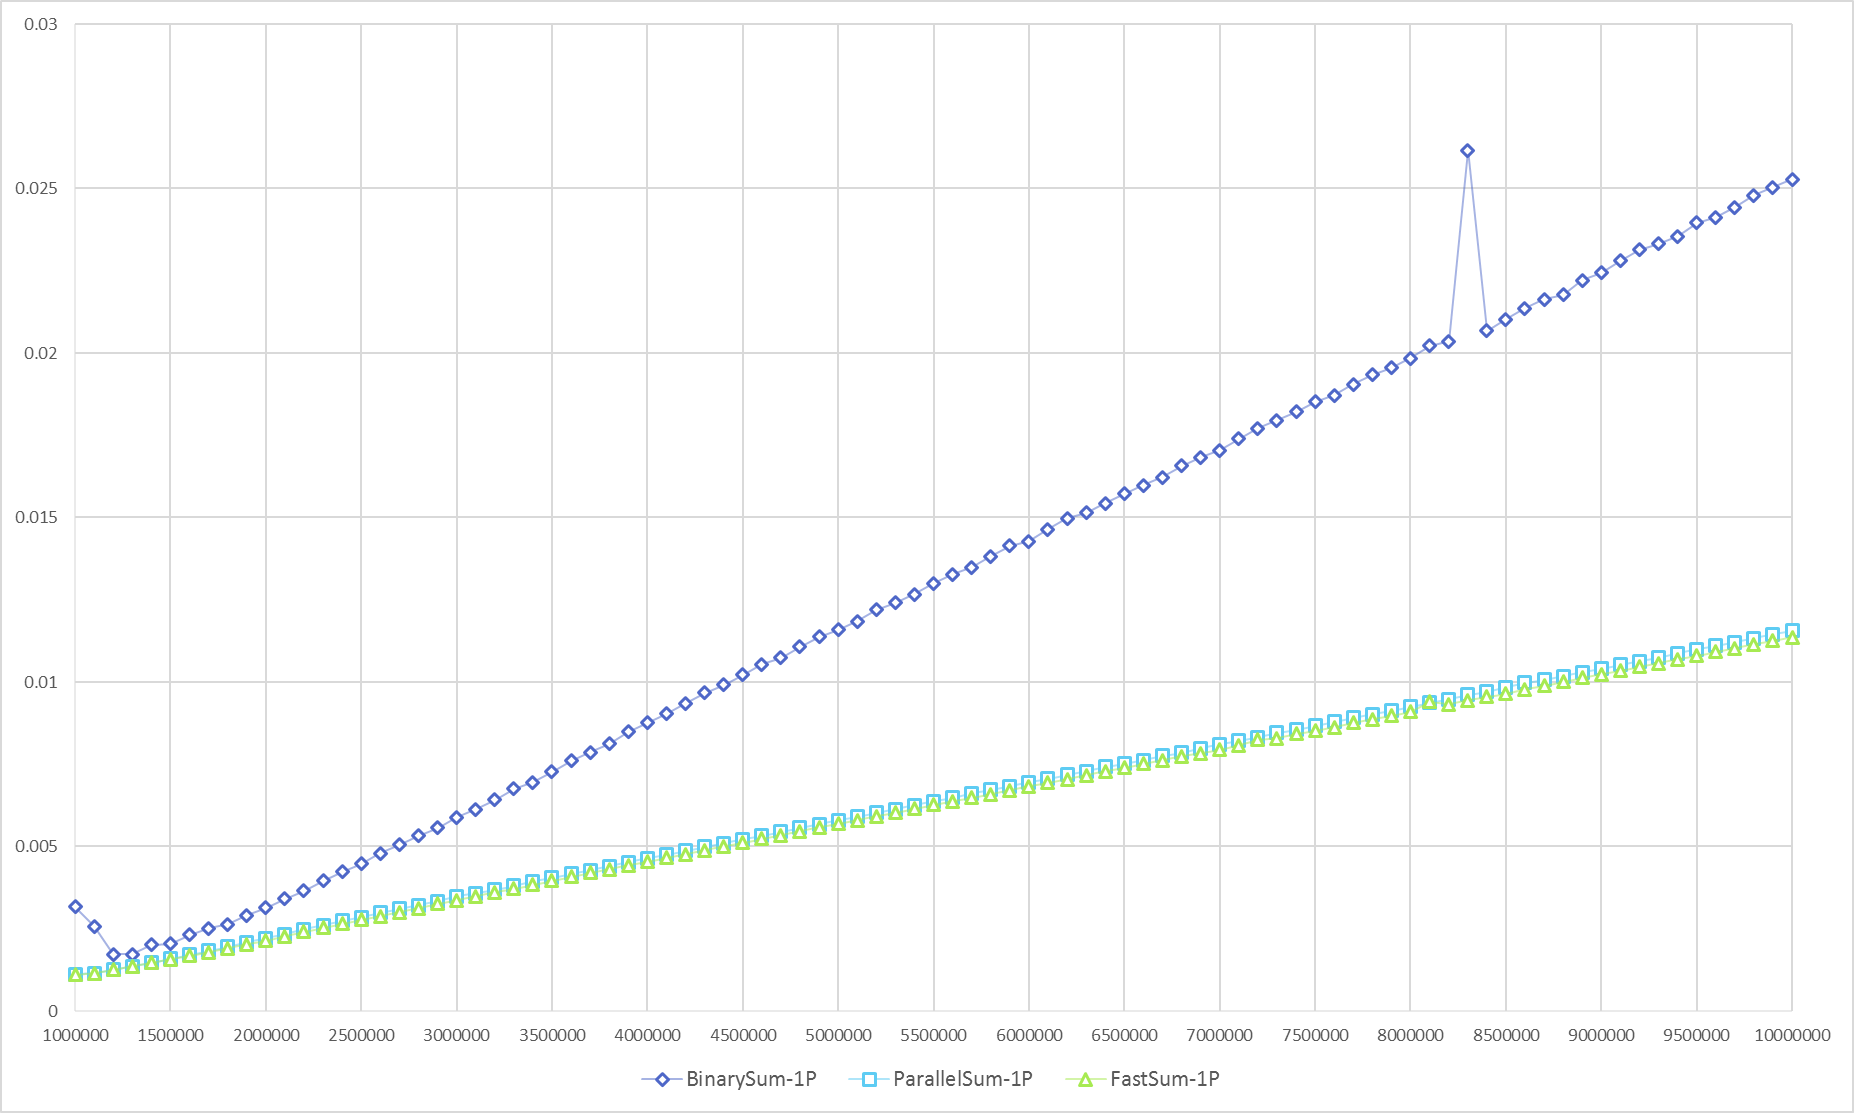
\includegraphics[width=\textwidth]{1_thread.png}
	\caption{Single Thread Performance}
\end{figure}

The final chart shows the performance of each method when using 16 threads, as this number of threads produced the best performance. We can see, again that the management required for the binary sum creates a very large disparity between the runtimes when compared to the other two methods. At the largest value of N, the runtime of the binary sum is $\approx 3.64x$ that of the manually managed divide-and-conquer method and $\approx 5.79x$ of the fast sum runtime.
\begin{figure}[H]
	\centering
	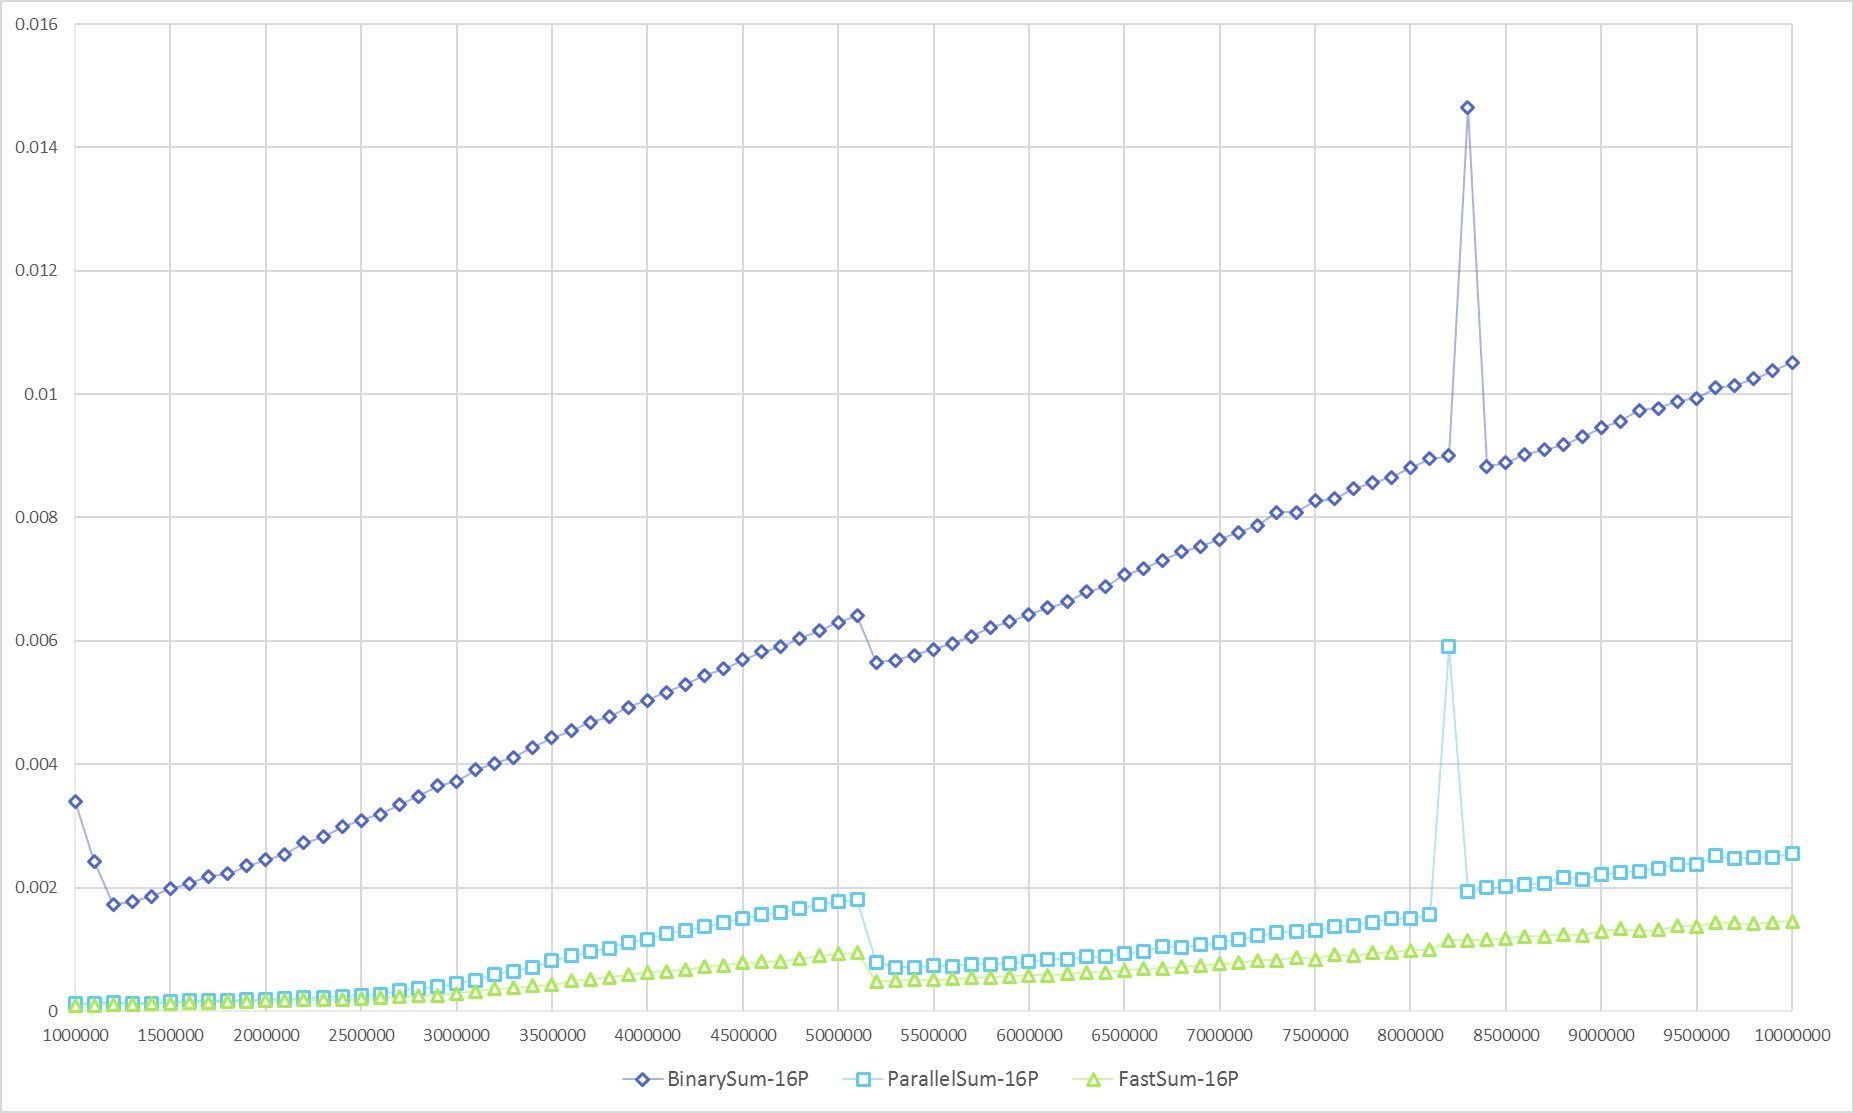
\includegraphics[width=\textwidth]{16_threads.png}
	\caption{16 Threads Performance}
\end{figure}

\section*{Conclusion}

Although we know the theoretical limit of the binary sum to be $O(log_2 N)$, in practice the actual parallel performance is closer to that of the serial performance. Even at small values of N, which we could realistically have more processors than data points, the standard parallel sum may actually run faster due to the amout of overhead it takes to create the scratch space for the binary tree sum method.

%====================================================================
\newpage
\section*{Code Appendix}
\lstinputlisting[language=C++]{../main.cpp}

\end{document}